%%%%%%%%%%%%%%%%%%%%%%%%%%%%%%%%%%%%%%%%%%%%%%%%%%%%%%%%%%%%%%%%%%%%%%%%%%%%%%%%
\chapter{Архитектура системы и выбор средств разработки}

Для расширения возможностей анализа CRM-системы с помощью интеграции платформы Pentaho, необходимо предоставить доступ к результатам OLAP-анализа Pentaho BI.

\section{Получение отчёта с сервера Pentaho}

Для начала, необходимо получить отчёт с сервера. Самый простой способ - выгрузка вручную. В пользовательской консоли пользователь может осуществлять взаимодействие с файлами. Пример такого взаимодействия демонстрирует рисунок \ref{fig:load_analysis}.

\begin{figure}[htbp]
	\centering
	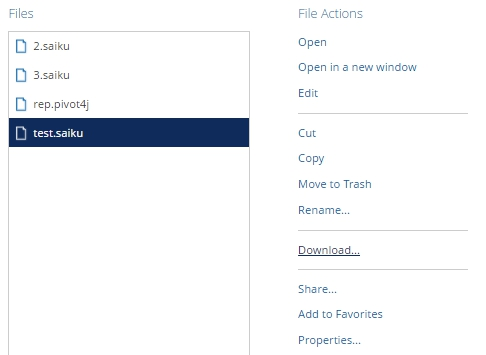
\includegraphics[width=.9\textwidth]{fig/chapter_3/load_analysis}
	\caption{Загрузка отчёта с помощью консоли}
	\label{fig:load_analysis}
\end{figure}

Другой способ - это Kettle трасформации. Kettle или Pentaho Data Integration - это компонент платформы Pentaho, отвечающий за процесс Извлечения, Преобразования и Выгрузки данных (ETL). С помощью таких операций можно осуществлять передачу данных между клиентом и сервером. Однако, Kettle требует изучения.

Ещё один способ - использование Pentaho API \cite{pentahoDocs}. В нём имеется набор точек входа, URL для доступа к ресурсам сервера, позволяющих работать с источниками данных и файлами, находящимися на сервере. Пример URL для получения списка файлов и возвращаемый список можно увидеть в листинге \ref{listings:get_files}.

\begin{lstlisting}[
label={listings:get_files},
caption={"Команда получения списка файлов выбранной директории Pentaho API"},
style=Java]
GET /pentaho/api/repo/files/:home:admin/children
\end{lstlisting}

Сам список файлов передаётся в формате XML. Пример списка представлен в листинге \ref{listings:fileTree}.

\begin{lstlisting}[
label={listings:fileTree},
caption={"Пример файлового древа"},
style=Java]
<repositoryFileTreeDto>
	<children>
		<file>
			<createdDate>1405356318621</createdDate>
			<fileSize>-1</fileSize>
			<folder>true</folder>
			<hidden>false</hidden>
			<id>fileId;/id>
			<locale>en</locale>
			<locked>false</locked>
			<name>admin</name>
			<ownerType>-1</ownerType>
			<path>/path/to/dir</path>
			<title>admin</title>
			<versioned>false</versioned>
		</file>
	</children>
</repositoryFileTreeDto>
\end{lstlisting}

В параметрах запроса можно добавить фильтр. Пример запроса с фильтром приведём в листинге \ref{listings:filter}.

\begin{lstlisting}[
label={listings:get_files},
caption={"Команда получения списка файлов выбранной директории Pentaho API"},
style=Java]
GET /pentaho/api/repo/files/:home:admin/children?filter=*.saiku
\end{lstlisting}

Плагины в Pentaho могут выполнять следующие функции:

\begin{enumerate}
	\item Обслуживание другого приложения;
	\item Визуализация данных в новом формате;
	\item Регистрация новых управляющих файлов в движке и в пользовательской консоли;
	\item Интегрирование BI сервера со сторонними приложениями;
	\item Изменение пользовательской консоли.
\end{enumerate}

Для интеграции Vtiger СRM с Pentaho BI необходим REST-сервис, обозначенный в пункте 1. Взаимодействие с пользователем будет осуществляться через веб-интерфейс

\section{REST API сервис}

REST (сокр. от англ. Representational State Transfer — «передача состояния представления») — это стиль архитектуры программного обеспечения для распределенных систем, таких как World Wide Web, который, как правило, используется для построения веб-служб.\cite{rest}

REST приложения используют методы протокола HTTP:

\begin{itemize}
	\item GET - возвращает выбранный ресурс;
	\item POST - создаёт ресурс на сервере;
	\item PUT - обновляет указанный ресурс. Также используется в качестве аналога POST для создания;
	\item DELETE - удаляет указанный ресурс.
\end{itemize}

Pentaho API использует модель REST и технологию точек входа для доступа к данным. Точки входа позволяют соотнести URI и нужный HTTP метод. Иными словами, - это URL-ссылка, которую приложение-клиент будет использовать для общения с REST-сервисом.

На рисунке \ref{fig:structure} приведена архитектура разрабатываемого приложения. Пользователь посредством web-интерфейса выбирает имеющийся на сервере Pentaho отчёт. После чего, приложение получает отчёт с сервера. Пользователь, выделив поля заголовков, может сгенерировать ссылку для получения выделенных данных извне через REST-сервис. К REST-сервису можно обращаться для получения доступа к элементам отчёта, при помощи HTTP-запроса. 

\begin{figure}[htbp]
	\centering
	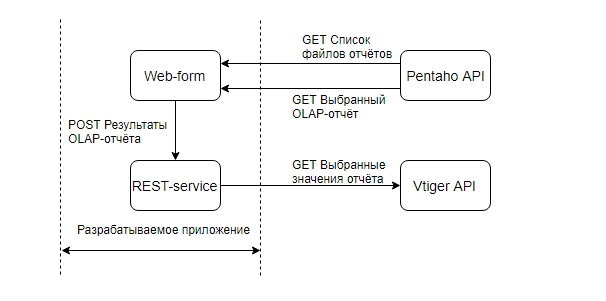
\includegraphics[width=.9\textwidth]{fig/chapter_3/structure}
	\caption{Архитектура разрабатываемого приложения}
	\label{fig:structure}
\end{figure}

\section{Выбор средств разработки}

Для разработки сервиса предоставлено две воможности: разработка на языке Java, либо разработка с помощью Pentaho Plugin Builder(SPARKL).

\subsection{Java}

Разработка плагина на языке Java ведётся на основе фреймворков Spring и JAX-RS. При помощи этих инструментов возможно разработать REST-приложение, основанное на аннотациях и XML-конфигурации зависимостей классов. 

Необходимы навыки программирования на языке Java, понимание технологии Модель-Представление-Контроллер. При этом, нет необходимости в изучении CTools и DI. Это также даёт возможность работать в более удобной разработчику среде разработки.

Плагин, написанный на Java, обычно является REST-сервисом, запускающимся при старте сервера Pentaho и работающем на том же домене. Такому сервису задаётся URL-адрес, и в момент обращения к точке входа плагина сервер принимает запрос, идентифицирует пользователя и сам обращается к сервису.

\subsection{Sparkl}

Sparkl, также являясь плагином для Pentaho сервера, позволяет создавать плагины и приложения для Pentaho. Разработанный на Sparkl плагин является объединением наборов CDE(приборных панелей) и Kettle(Pentaho Data Integration) работ и трансформаций. 

Достоинством такого способа является прямое взаимодействие с данными и файлами сервера, что обеспечивает высокую скорость работы при обработке больших объёмов данных. Однако, для создания плагина необходимы знания Pentaho Data Integration и умение работы с контрольными панелями.

\section{Разбор JSON объекта}



\section{Итоги}

Были рассмотрены решения для создания плагина Pentaho BI. Разработка на языке Java является более предпочтительным выбором разработчику ПО, так как не требует дополнительных инструментов и знаний со стороны BI. Java также удовлетворяет требованиям минимизации необходимых для установки средств платформы Pentaho. 

Sparkl, в свою очередь, требует изучения таких средств и инструментов, как CDE и Kettle. Однако, данный вариант будет более подходящим вариантом людям, не имеющим опыта разработки ПО.

%%%%%%%%%%%%%%%%%%%%%%%%%%%%%%%%%%%%%%%%%%%%%%%%%%%%%%%%%%%%%%%%%%%%%%%%%%%%%%%%